\section{Introduction}

The big picture
\\
 \begin{itemize}
 	\item Understanding the flow in wind parks can have a valuable impact on many fields
 	\begin{itemize}
 		\item Engineering: Optimize turbine design and control to minimize load while maximizing power output
 		\item Economics: Assess the economic viability
 		\item Environment and Policy: Impact on the local environment and how to regulate it
 	\end{itemize}
 	\item While the detailed, high-fidelity simulation of turbines is computationally very expensive, low-fidelity engineering models present an alternative
 	\item Model the physical phenomena in a simplified way to represent the most important aspects for the problem at hand
 	\item A popular engineering model for wind turbines is the Actuator Line Method
 	\item Turbine tower and blades are represented as slender beams
 	\item Allows the detailed study of wake effects and blade deformations
 	\item Open-source tool OpenFAST implements such models
 	\item Coupling OpenFAST with a high-fidelity LES CFD solver would allow to accurately solve the wind field at moderate computational cost \ref{fig:openfast:coupling}
 	\item preCICE is a multi-physics coupling library to couple different solvers
 	\item Coupled tools include OpenFOAM, an open-source CFD solver used in industry and academia
 	\item To couple a tool via preCICE, an additional piece of software called adapter is necessary
 	\item Idea: Write a preCICE-OpenFAST adapter to couple OpenFAST to CFD solvers via preCICE
 	\\
 \end{itemize}

\begin{figure*}[h]
	\centering
	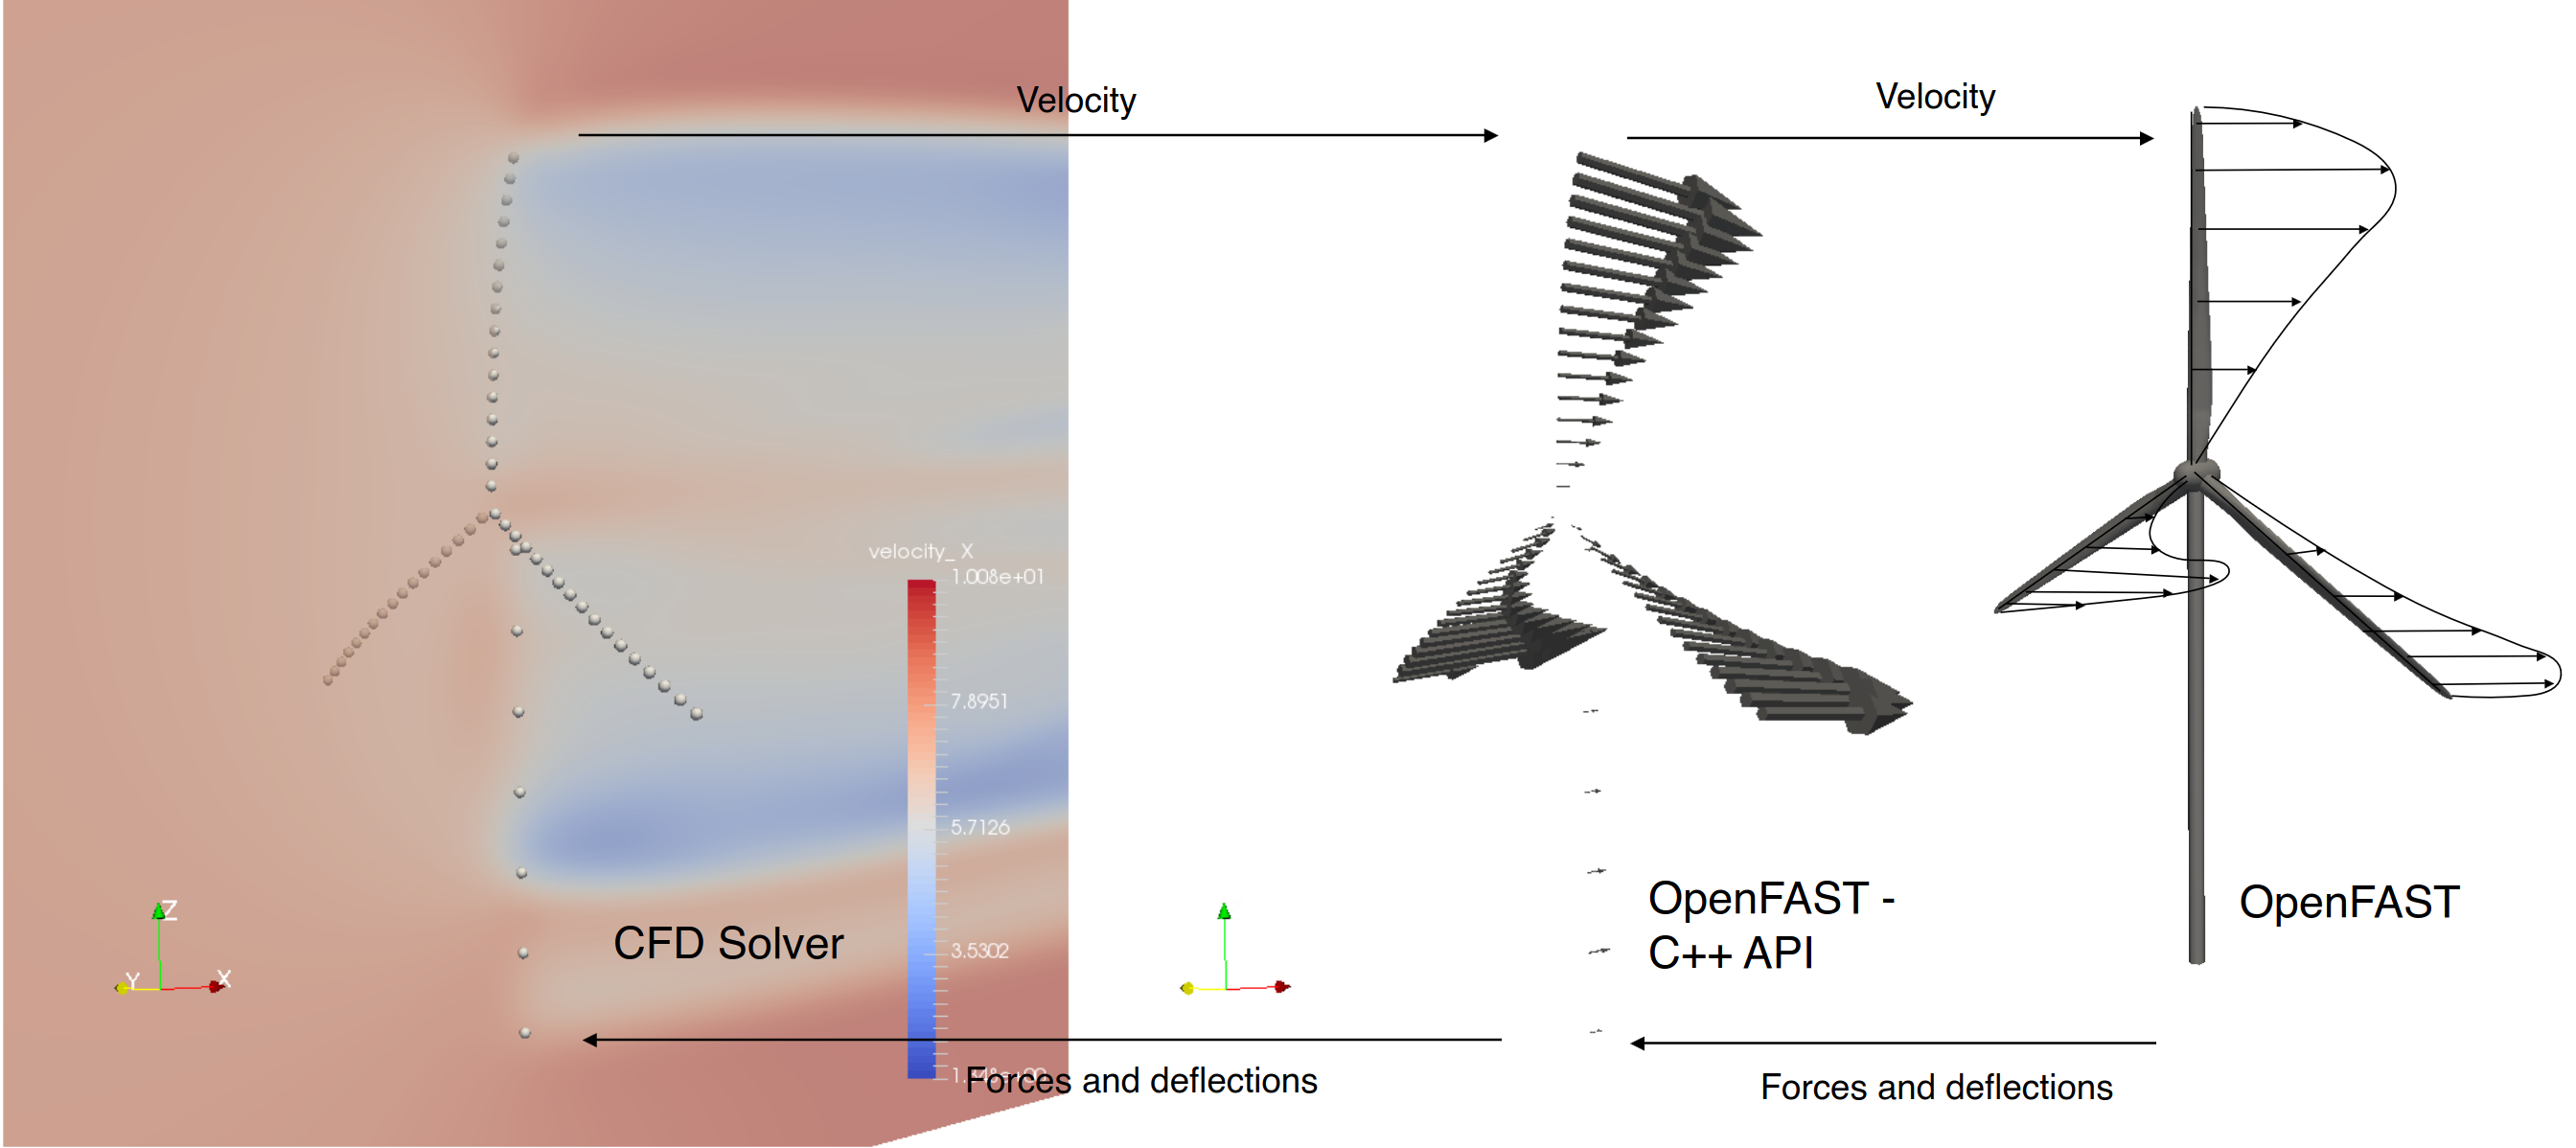
\includegraphics[width=0.9\textwidth]{images/openfast-coupling-scheme.png}
	\caption{Coupling of OpenFAST to a CFD program. The fluid solver computes the flow dynamics and sends velocity data to OpenFAST. OpenFAST simulates the turbine dynamics and sends back forces and deflections, which are imposed on the flow field. Source: OpenFAST documentation\protect\footnotemark}
	\label{fig:openfast:coupling}
\end{figure*}

\footnotetext{{\url{https://ganesh-openfast.readthedocs.io/en/latest/_images/actuatorLine_illustrationViz.pdf}(visited on 07.11.2023)}}

Literature Review: Understand what has been done already to couple OpenFAST with CFD solvers and how our approach relates to that
\\
\begin{comment}
	

\textbf{OF2: A coupling library for OpenFOAM}
\begin{itemize}
    \item Motivation: Model FOWTs with mixed fidelity to speed up the design process
    \item OpenFOAM computes the floater hydrodynamics with high fidelity
    \item OpenFAST computes the rotor aerodynamics and servo-elastic response in low-fidelity
    \item Method: Two OpenFOAM libraries perform the coupling
    \item libForcedOpenFAST: Software layer to interact with and execute OpenFAST
    \item libOF2: Software layer to read and write data from OpenFOAM
    \item Both libraries communicate with each other
    \item Benefits: Less computationally expensive than CFD only, simulation of large turbine displacements (drift, rotation) possible
    \item Drawbacks: Done for hydrodynamics (OpenFOAM replaces HydroDyn), not sure if this approach would work for aerodynamics as well (yes)
    \\
\end{itemize}

\end{comment}

\textbf{AspFAST} \cite{Taschner:2022}
\begin{itemize}
	\item Motivation
	\begin{itemize}
		\item Wind farm simulation combines the analysis of large-scale flow dynamics with individual turbine behavior
		\item Different tools are needed to model these two phenomena
		\item AspFAST couples the LES code GRASP with the wind turbine tool OpenFAST to perform such simulations
	\end{itemize}
	\item Methodology
	\begin{itemize}
		\item AspFAST is a binder code between the GPU-driven GRASP and the CPU-driven OpenFAST
		\item OpenFAST is accessed via C++ API → AspFAST is the driver code
		\item AspFAST takes care of the mapping and communication between the tools
	\end{itemize}
	\item What AspFAST does
	\begin{itemize}
		\item Synchronize GRASP and OpenFAST
		\item Exchange data: Force, Velocity, Position (of the turbine blades)
		\item Map data and make use of the actuator line model
		\begin{itemize}
			\item Map velocity from GRASP to OpenFAST
			\item Map force from OpenFAST to GRASP
			\item Make use of both internal meshes inside of OpenFAST
		\end{itemize}
	\end{itemize}
	\item How it relates to our idea
	\begin{itemize}
		\item Very close to what we want to achieve
		\item Difference: GRASP is a commercial and licensed software, AspFAST allows coupling only to this one solver
		\item The coupling of the parallel flow solver NaluWind with OpenFAST pursues a very similar idea
		\\
	\end{itemize}
\end{itemize}


\textbf{foamFAST and MPCCI coupling tool} \cite{Weber:2017}
\begin{itemize}
	\item Motivation
	\begin{itemize}
		\item Replace the low-fidelity aerodynamic calculations in FAST, based on the BEM theory, with high-fidelity calculations in OpenFOAM
		\item BEM theory is not sufficient for many applications; CFD is needed
		\item Use the coupling tool MpCCI to perform the coupling
	\end{itemize}
	\item Methodology
	\begin{itemize}
		\item Couple OpenFOAM and OpenFAST via the coupling tool MpCCI
		\item MpCCI is a licensed coupling tool for partitioned multi-physics simulations developed by the Fraunhofer SCAI
		\begin{itemize}
			\item Connect tools to MpCCI via adapters
			\item Once the adapter is written, you can couple your tool to any other tool connected to MpCCI
			\item MpCCI acts as the master algorithm
		\end{itemize}
		\item This project developed an OpenFAST adapter from scratch and adapted an existing OpenFOAM adapter to perform the coupling
		\item Source code is not violated
	\end{itemize}
	\item How it relates to our idea
	\begin{itemize}
		\item Very similar approach to preCICE´
		\item Difference of MpCCI and preCICE: preCICE takes the library approach, while MpCCI takes the master algorithm approach
		\item MpCCI is commercial and has limited HPC capabilities
		\\
	\end{itemize}
\end{itemize}


\textbf{SOWFA} \cite{Churchfield:2012}
\begin{itemize}
	\item Developed by NREL
	\item Simulator for Wind Farm Applications based on OpenFOAM
	\item Enables a coupling with OpenFAST
	\item Methodology
	\begin{itemize}
		\item Implements a turbine class horizontalAxisALM in OpenFOAM to call OpenFAST and exchange data
		\item This class can be included in any OpenFOAM solver
		\item The solver calls OpenFAST during each timestep
	\end{itemize}
	\item How this relates to our idea
	\begin{itemize}
		\item Different approach: Is based on the modification of OpenFOAM source code while we strive to leave the solvers untouched
		\item A lot of internal OpenFOAM knowledge necessary
		\\
	\end{itemize}
\end{itemize}

\textbf{ExaWind: A Coupling of NaluWind with OpenFAST} \cite{Sprague:2019}\\
\begin{itemize}
	\item NaluWind is an open-source massively parallel, incompressible flow solver for wind turbines and parks
	\item Is a wind-focused adaption of the general flow solver NaluCFD
	\item Focus on delivering flow simulations in exascale
	\item Coupled to OpenFAST to perform multi-fidelity simulations of wind parks
	\item Verified simulation on single turbine case against other codes and experiments
	\item Emphasis on scalability and increased simulation speed through advanced solver and coupling algorithms and the optional use of GPUs
	\item Extensive documentation with insights into the theory and verification 
	\item How does it relate to our work
	\begin{itemize}
		\item Very close to what we want to do
		\item Especially interesting for high-performance applications
		\item Expert tool that needs some time to set up, understand, and run --> The hope is that our coupling to the "standard" tool OpenFOAM will have a lower barrier for beginners
	\end{itemize}
\end{itemize}

Given the previous work, why should we continue to develop a preCICE-OpenFAST adapter?
\begin{itemize}
	\item Combines positive aspects of previous works while avoiding some drawbacks
	\item Maintainability: Adapter is a separated piece of code which is easier to maintain than a modified OpenFOAM solver
	\item Open access: No license
	\item Plug and play: Adapter opens the road to connect OpenFAST not only to OpenFOAM, but to any CFD solver coupled to preCICE
	\item Easy to use: preCICE creates a clean simulation environment, seperating the coupled tools clearly, from which students and professionals benefit
\end{itemize}
What are some serious drawbacks?
\begin{itemize}
	\item There are currently no preCICE adapters for other CFD solvers that would be interesting to couple to: NaluWind, GRASP, ...
	\item Developing such adapters would mean to re-implement a functionality that already exists in native coupling tools --> questionable if that is a good investment
\end{itemize}
